El objetivo de esta sección es dar una introducción a los corpus utilizados, junto con la teoría referente a las metodologías utilizadas para su procesamiento. Los detalles implementativos serán descriptos más adelante en la Sección \ref{herramientas}.

\subsection{Primer corpus en castellano} \label{firstCorpus}

Al inicio de la investigación, comenzamos con el corpus \textit{SECYT-mujer}, construido por el Laboratorio de Investigaciones Sensoriales (INIGEM, UBA-CONICET) \cite{secytMujer}. El mismo está compuesto por $741$ oraciones cortas declarativas habladas por una locutora profesional en castellano rioplatense, equivalentes a $48$ minutos de habla. A continuación, tres ejemplos de las oraciones articuladas por la locutora:

\indent\indent \textit{La voluntad del juez fue impuesta en tribunales.}

\indent\indent \textit{Los vinos uruguayos han mejorado en el último lustro.}

\indent\indent \textit{Al atardecer se puso su disfraz juglaresco.}

En la Figura \ref{pipeline} presentamos el esquema general para en entrenamiento de un HMM que utilizaremos a lo largo de todo el trabajo. En primer lugar extraemos las caracteristicas acusticas del corpus (exitation parameters y spectral parameters en la figura) y generaremos el etiquetado fonético. Estos serán utilizados para entrenar el modelo. Por último, una vez generado el modelo se procede a la etapa de sintesis donde tomamos el HMM y una nueva transcripción para generar los parametros acusticos necesarios para producir el nuevo audio.

\begin{figure}
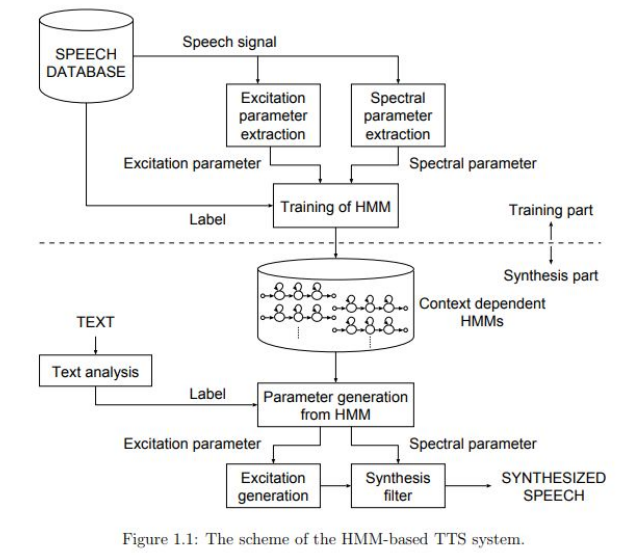
\includegraphics[scale=0.5]{imagenes/pipeline.png}
\centering
\caption{Esquema de un sistema TTS basado en HMM (tomado de \cite{phoneticAndProsodic}, página 18)}
\label{pipeline}
\end{figure}

Comenzamos entonces construyendo el etiquetado fonético para el corpus. Estos etiquetados consistirán en una lista de fonos donde se indica cuándo comienza y termina cada uno en el audio. La calidad de las oraciones que logremos sintetizar a posteriori dependerá fuertemente del etiquetado, por lo que es necesario prestar especial cuidado en que las transcripciones estén lo mejor alineadamente posible con los audios. Las transcripciones serán necesarias para entrenar los modelos de HMM+GMM, extrayendo tanto la información acústica para cada fono (cosas tales como la frecuencia principal, la duración, etc), como así también información contextual (por ejemplo: cómo suena un fono cuando está seguido de algún otro, al principio de una oración, si se encuentra en un diptongo, etc). Por ende, una mala transcripción se traducirá indefectiblemente en un mal modelo y malas oraciones sintetizadas. Llevamos a cabo varias pruebas de concepto utilizando HTS en este corpus, experimentando con diversos métodos para obtener el etiquetado fonético. 

La primera estrategia consistió en utilizar alineamiento automático con \textit{EHMM alignment} \cite{phoneticCapturing} empleando Festival y Festvox. Esta técnica tiene como principal ventaja su sencillez. Para generar las transcripciones solo es necesario contar con el corpus que se quiere anotar y sus \textit{transcripciones grafémicas} (Transcripciones gráficas, escritas).

Los resultados preliminares con este método fueron bastante negativos: los audios generados resultaban poco inteligibles notándose claros defectos acústicos, el más notable siendo el fono [\textipa{r}] (\textit{perro}) que se asemejaba más a [\textipa{R}] (\textit{pero}).

Utilizando la herramienta de visualización y manipulación de audio Praat \cite{praat} para visualizar el alineamiento entre las transcripciones fonéticas y los audios, descubrimos que la alineación de algunas oraciones estaba desfasada algunas milésimas de segundo respecto de los audios. Dado que para el alineamiento automático es necesario alinear los audios del corpus con audios sintetizados con Festival, sospechamos que pudo haber problemas con la calidad del corpus o que los audio sintetizados por Festival eran demasiado disímiles comparados con los audios reales. 

Dado que para el corpus contamos con las transcripciones fonéticas anotadas de manera manual, procedimos a implementar un híbrido, que consiste en tomar los tiempos de las anotaciones fonéticas manuales y la información contextual y el repertorio fonético generado a partir del proceso de EHMM y combinarlos en una nueva transcripción fonética. De esta manera buscamos mejorar la alineación, utilizando en teoría una transcripción más precisa, pero manteniendo el repertorio fonético y la misma meta-información brindada por el alineamiento automático. Mantener el mismo repertorio fonético y meta-información de las transcripciones será clave para la síntesis de audios. Esto nos permitirá utilizar Festival para generar las ``partituras'' que queramos sintetizar y que éstas tengan los mismos símbolos fonéticos (Para más información ver Sección \ref{phoneMaping}).

El modelo generado con estas transcripciones mixtas resultó superior a los generadas solo con alineamiento automático. Aún así los audios sintetizados todavía no alcanzaron una calidad aceptable, realizando pruebas notamos que el sonido resultaba metálico y las frases poco inteligibles. Además se pudo percibir de manera informal otros detalles tales como que la voz original tenía un pitch mayor que la producida por los modelos, alrededor de un $10\%$.

Para intentar mejorar la calidad de los audios en este punto sumamos otro corpus de datos en castellano.

\subsection{Segundo corpus en castellano}

En este punto de la investigación obtenemos un segundo corpus de datos, también contribuido por el Laboratorio de Investigaciones Sensoriales, \textit{loc1\_pal} \cite{loc1pal} con $1593$ oraciones cortas con una mezcla entre frases declarativas e interrogativas del $80\%$ y $20\%$ aproximadamente, pronunciadas por una locutora profesional con acento rioplatense con aproximadamente $2$ horas y $26$ minutos de habla. Con este nuevo conjunto de datos esperamos conseguir mejores resultados.

Presentamos tres ejemplos de las oraciones articuladas por la locutora:

\indent\indent \textit{Álvarez se había animado a contarle un chiste.}

\indent\indent \textit{Alzó la voz para ahuyentar a los perros.}

\indent\indent \textit{Ayer el general cumplió ochenta años.}

También vale la pena aclarar que algunas de las oraciones del primer y el segundo corpus están duplicadas. Por ejemplo la primera oración de ejemplo también estaba presente en \textit{secyt-mujer}.

Para este corpus no contábamos con transcripciones fonéticas manuales por lo que nos vimos forzados a utilizar EHMM nuevamente. Aún así, los resultados fueron superiores a los conseguidos con \textit{secyt-mujer}. Al contrario que en \textit{secyt-mujer}, al visualizar este corpus con Praat, no pudieron apreciarse mayores desfasajes entre las transcripciones fonéticas y los audios.

Además los audios sintetizados resultaban inteligibles y con un marcado acento rioplatense. Tras algunas pruebas de concepto donde se experimentó con varios parámetros modificables dentro de HTS, logramos obtener resultados que superaban de manera significativa aquellos obtenidos previamente con \textit{secyt-mujer}. Por consiguiente consideramos que los audios generados habían alcanzado una buena calidad que resultara ininteligible y aceptable para el objetivo de la investigación, por lo que decidimos utilizar uno de estos modelos para el resto del trabajo.

%pag 28 htbook:
%The single biggest problem in building context-dependent HMM systems is always data insuffi-
%ciency. The more complex the model set, the more data is needed to make robust estimates of its

Especulamos que la disparidad en la calidad de los resultados es causada principalmente por la cantidad de audios y horas de habla de cada corpus \cite{phoneticAndProsodic}. Consideramos que esto juega un papel predominante en la calidad de los sistemas TTS generados, aún cuando se utiliza un método de etiquetado puramente automático y propenso a errores sistemáticos en el alineamiento.

%Finalmente necesitamos generar otra voz con un idioma diferente que nos permita interpolar con el modelo previamente detallado. Para esto utilizamos el corpus

\subsection{Corpus en inglés}

Por otro lado entrenamos una voz en inglés utilizando el corpus \textit{CMU-ARCTIC-SLT} \cite{cmuArtic} con $1132$ oraciones en inglés y $56$ minutos de habla articuladas por una mujer estadounidense, disponible en la página de HTS \cite{hts}. Ya que este corpus venía a modo de demo con HTS, asumimos que los parámetros de entrenamiento y las transcripciones fonéticas habían sido seleccionadas de manera apropiada, por lo que no intentamos mejorar la calidad de las transcripciones fonéticas más allá de lo que los scripts ofrecían. 

Una vez más realizamos pruebas perceptuales informales para tener una idea cualitativa de los modelos generados. Los audios en inglés sintetizados con este modelo resultan inteligibles y con buena pronunciación. Sin embargo, en oraciones extensas, por ejemplo en audios de $17$ segundos, pueden empezar a notarse errores más graves en la prosodia. La misma se torna monótona y con ella, la inteligibilidad de los audios disminuye.

Presentamos tres ejemplos de las oraciones articuladas por la locutora:

\indent\indent \textit{Author of the danger trail, Philip Steels, etc.}

\indent\indent \textit{Not at this particular case, Tom, apologized Whittemore.}

\indent\indent \textit{For the twentieth time that evening the two men shook hands.}

En la Sección \ref{entrenamientoHTS} detallaremos más detenidamente los aspectos técnicos de los corpus utilizados.

% hablar de intelibililidad como para ya ir adelantando el tema
% Cosas para hablar:
% 5 fonos.
%TODO: phonetically balanced?
% desarrollar generacion de uternaces: secty alineaminento mixto: tiempos a mano, features automaticos.
